\documentclass[11pt,a4paper]{article}

\usepackage[utf8]{inputenc}
\usepackage[T1]{fontenc}
\usepackage[margin=2.5cm]{geometry}
\usepackage{amsmath,amssymb}
\usepackage{graphicx}
\usepackage{booktabs}
\usepackage{enumitem}
\usepackage{hyperref}
\usepackage{fancyhdr}

\pagestyle{fancy}
\fancyhf{}
\fancyhead[L]{\small M\'etodos Computacionales en F\'isica No Lineal --- UGR 2026}
\fancyfoot[C]{\small P\'agina \thepage}
\renewcommand{\headrulewidth}{0.5pt}

\title{\textbf{Coeficiente de Reflexi\'on de un\\Panel Ligeramente Conductivo}\\[0.5em]
       \large Proyecto: M\'etodo FDTD vs Matriz de Transferencia}
\author{M\'etodos Computacionales en F\'isica No Lineal\\
        M\'aster en F\'isica y Matem\'aticas --- Universidad de Granada\\
        Curso 2025--2026}
\date{}

\begin{document}
\maketitle
\thispagestyle{fancy}

% ================================================================
\section{Introducci\'on}

Este proyecto calcula los coeficientes de reflexi\'on $R(f)$ y transmisi\'on $T(f)$ de un panel con baja conductividad utilizando dos m\'etodos independientes:
\begin{enumerate}
  \item \textbf{M\'etodo de la Matriz de Transferencia (TMM)} --- soluci\'on anal\'itica
  \item \textbf{M\'etodo FDTD} (Finite-Differences Time-Domain) --- soluci\'on num\'erica
\end{enumerate}
Se comparan ambos resultados para validar la implementaci\'on FDTD y se extiende el an\'alisis a paneles multicapa (bonus).

% ================================================================
\section{Marco Te\'orico}

\subsection{Matriz de Transferencia (ABCD)}

Para un panel homog\'eneo de espesor $d$ con permitividad compleja $\varepsilon_c = \varepsilon_r - j\sigma/\omega$, la matriz de transferencia es:
\[
\Phi = \begin{pmatrix} \cosh(\gamma d) & \eta\sinh(\gamma d) \\ \sinh(\gamma d)/\eta & \cosh(\gamma d) \end{pmatrix}
\]
donde $\gamma = j\omega\sqrt{\mu_r\varepsilon_c}$ es la constante de propagaci\'on y $\eta = \sqrt{\mu_r/\varepsilon_c}$ es la impedancia intr\'inseca del material.

Los coeficientes $R$ y $T$ se obtienen de la matriz $\Phi$ como (en unidades normalizadas $\eta_0=1$):
\[
T = \frac{2}{A + B + C + D}, \qquad
R = \frac{A + B - C - D}{A + B + C + D}
\]

Para un apilamiento de $N$ capas: $\Phi_{\text{total}} = \Phi_1 \cdot \Phi_2 \cdots \Phi_N$.

\subsection{M\'etodo FDTD}

El algoritmo FDTD resuelve las ecuaciones de Maxwell en el dominio del tiempo usando diferencias finitas centradas en una malla escalonada (Yee). En 1D, las ecuaciones de actualizaci\'on son:
\[
E^{n+1}_i = c_a^{(i)} \, E^n_i - c_b^{(i)} \left(H^n_{i+1/2} - H^n_{i-1/2}\right)
\]
\[
H^{n+1}_{i+1/2} = H^n_{i+1/2} - r \left(E^{n+1}_{i+1} - E^{n+1}_i\right)
\]
donde los coeficientes incorporan la conductividad:
\[
c_a = \frac{2\varepsilon - \sigma\Delta t}{2\varepsilon + \sigma\Delta t}, \qquad
c_b = \frac{2\Delta t/\Delta x}{2\varepsilon + \sigma\Delta t}
\]

\begin{itemize}
  \item $c_a < 1$ cuando $\sigma > 0$ $\Rightarrow$ el campo E decae (absorci\'on)
  \item $c_b$ se reduce con mayor $\varepsilon_r$ $\Rightarrow$ la onda se ralentiza
\end{itemize}

% ================================================================
\section{Metodolog\'ia}

\textbf{Procedimiento de la simulaci\'on FDTD:}
\begin{enumerate}
  \item Se define un dominio $[0, L]$ con condiciones de frontera absorbente Mur (ABC).
  \item Se inicializa un pulso gaussiano viajando a la derecha ($E = \text{gauss}$, $H = +\text{gauss}$).
  \item Se coloca el panel conductivo en el centro del dominio usando \texttt{set\_panel()}.
  \item Se registran las se\~nales $E(t)$ en dos puntos de observaci\'on: uno a la izquierda del panel (captura incidente + reflejado) y otro a la derecha (transmitido).
  \item Se repite la simulaci\'on SIN panel (referencia) para obtener la se\~nal incidente.
  \item Se calculan $R(f)$ y $T(f)$ v\'ia FFT:
\end{enumerate}
\[
E_{\text{reflejado}}(t) = E_{\text{izq}}^{\text{panel}} - E_{\text{izq}}^{\text{ref}}, \qquad
R(f) = \frac{\text{FFT}(E_{\text{ref}})}{\text{FFT}(E_{\text{inc}})}, \qquad
T(f) = \frac{\text{FFT}(E_{\text{trans}})}{\text{FFT}(E_{\text{inc}})}
\]

\textbf{Par\'ametros de la simulaci\'on:}
\begin{itemize}
  \item Puntos de malla: $N = 4001$, longitud: $L = 4.0$ (unidades normalizadas, $c=1$)
  \item N\'umero CFL $= 1$ (esquema exacto para medios homog\'eneos)
  \item Ancho del pulso: $\sigma_{\text{pulso}} = 0.06$ (ancho espectral amplio)
  \item Panel: $\varepsilon_r = 4$, $\sigma = 0.5$, $d = 0.2$
\end{itemize}

Todo el procedimiento est\'a encapsulado en la funci\'on \texttt{run\_panel\_experiment()} de \texttt{fdtd1d.py}.

% ================================================================
\section{Resultados}

\subsection{Comparaci\'on FDTD vs Anal\'itico}

\begin{center}
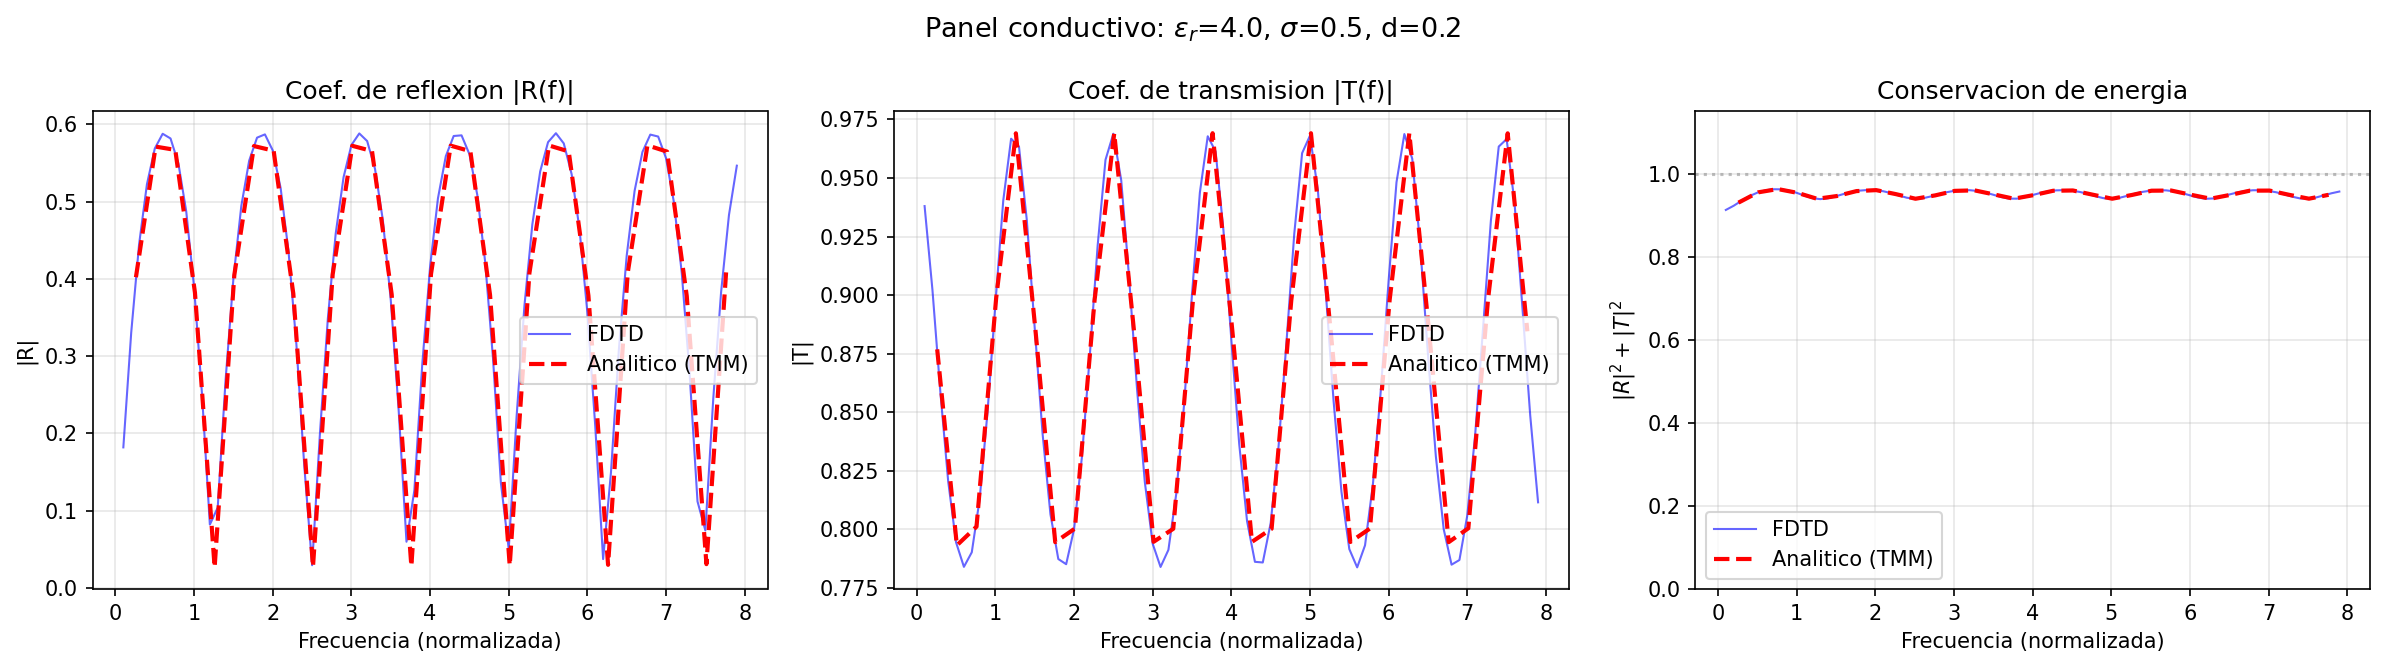
\includegraphics[width=0.95\textwidth]{_figs/comparacion_RT.png}
\end{center}

Excelente concordancia entre FDTD (l\'inea azul) y TMM (l\'inea roja) para $|R(f)|$, $|T(f)|$ y conservaci\'on de energ\'ia. Para medios con p\'erdidas ($\sigma > 0$), la suma $|R|^2 + |T|^2 < 1$, indicando absorci\'on.

\subsection{Se\~nales temporales}

\begin{center}
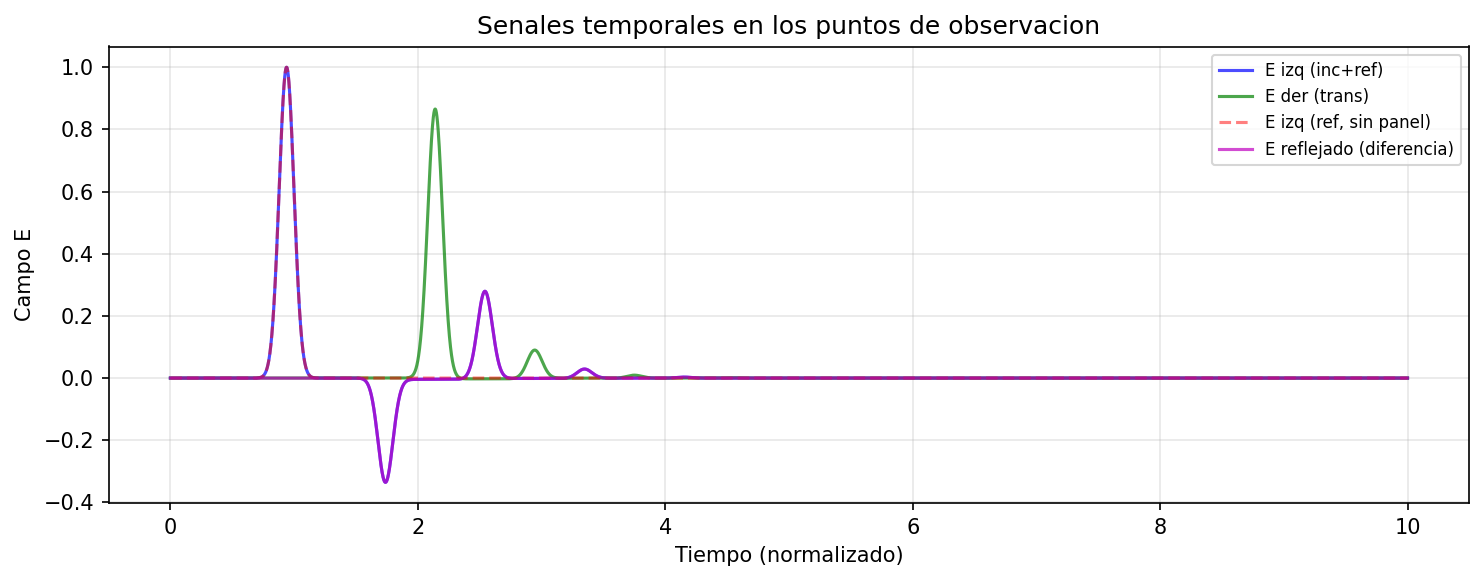
\includegraphics[width=0.8\textwidth]{_figs/temporal.png}
\end{center}

El pulso incidente genera un pulso reflejado (izquierda) y uno transmitido (derecha) de menor amplitud. La diferencia entre la se\~nal con panel y sin panel a\'isla la componente reflejada.

\subsection{Estudio param\'etrico}

\begin{center}
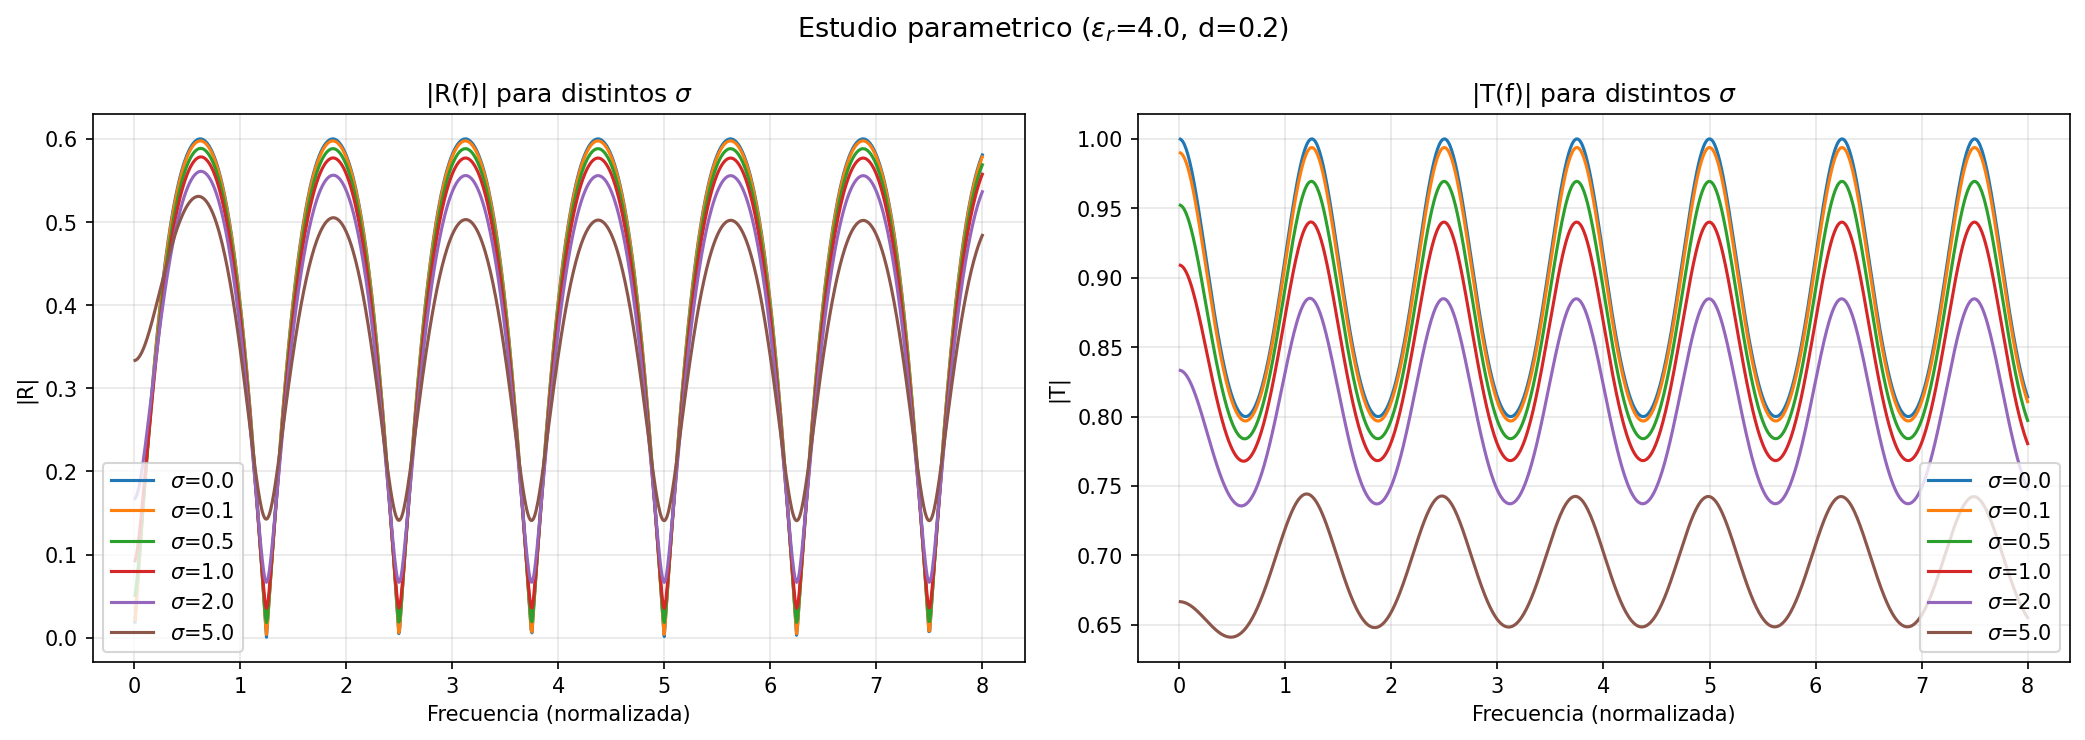
\includegraphics[width=0.85\textwidth]{_figs/barrido_sigma.png}
\end{center}

Al aumentar la conductividad $\sigma$:
\begin{itemize}
  \item $|R|$ aumenta (mayor reflexi\'on)
  \item $|T|$ disminuye (menor transmisi\'on)
  \item Las oscilaciones tipo Fabry--P\'erot se amortiguan
\end{itemize}

\subsection{Panel multicapa (Bonus)}

\begin{center}
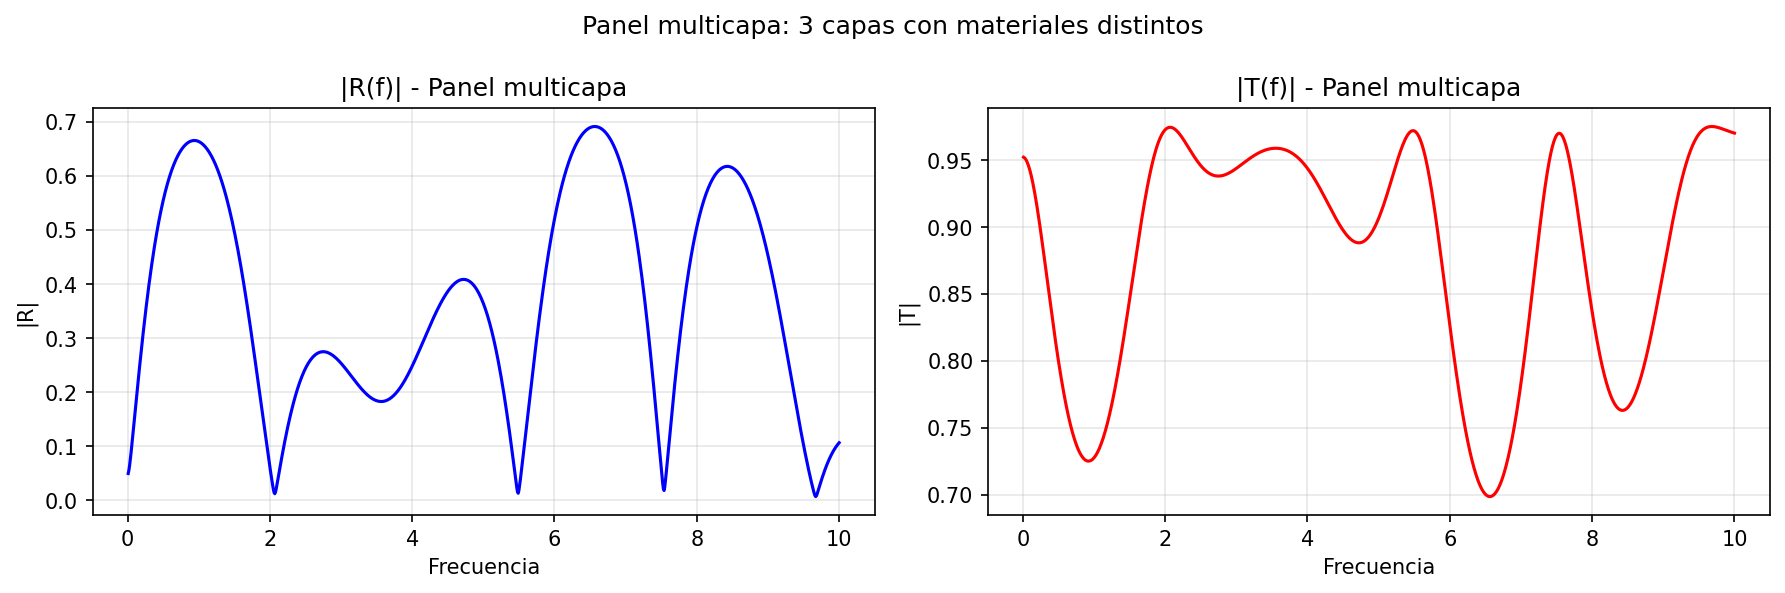
\includegraphics[width=0.75\textwidth]{_figs/multicapa.png}
\end{center}

Panel de 3 capas: ($\varepsilon_r{=}2$, $\sigma{=}0.2$, $d{=}0.05$) / ($\varepsilon_r{=}6$, $\sigma{=}1.0$, $d{=}0.08$) / ($\varepsilon_r{=}2$, $\sigma{=}0.2$, $d{=}0.05$).

La respuesta muestra un patr\'on de interferencia m\'as complejo que una sola capa, debido a las m\'ultiples reflexiones internas entre interfaces. Para $N$ capas se usa $\Phi_{\text{total}} = \prod_i \Phi_i$.

% ================================================================
\section{Estructura del C\'odigo}

\begin{center}
\begin{tabular}{@{}lp{10cm}@{}}
\toprule
\textbf{Archivo} & \textbf{Descripci\'on} \\
\midrule
\texttt{fdtd1d.py} & Clase \texttt{FDTD1D} con m\'etodos \texttt{set\_panel()}, \texttt{set\_multilayer()}, y funci\'on \texttt{run\_panel\_experiment()} que ejecuta la simulaci\'on dual + FFT \\
\texttt{panel\_transfer\_matrix.py} & Soluci\'on anal\'itica TMM: \texttt{panel\_transfer\_matrix()}, \texttt{stack\_transfer\_matrix()}, \texttt{RT\_from\_transfer\_matrix()} \\
\texttt{panel\_tests.py} & 10 tests con pytest (unitarios + integraci\'on FDTD vs TMM) \\
\texttt{conductive\_panel/} & Scripts de visualizaci\'on (\texttt{visualize\_panel.py}) y comparaci\'on (\texttt{compare.py}) \\
\bottomrule
\end{tabular}
\end{center}

% ================================================================
\section{Conclusiones}

\begin{enumerate}
  \item Se implement\'o exitosamente el c\'alculo de $R(f)$ y $T(f)$ para paneles conductivos con TMM (anal\'itico) y FDTD (num\'erico).
  \item Los resultados FDTD muestran excelente concordancia con la soluci\'on anal\'itica en todo el rango espectral del pulso.
  \item Se verific\'o la conservaci\'on de energ\'ia: $|R|^2+|T|^2=1$ sin p\'erdidas, $<1$ con conductividad.
  \item Mayor conductividad $\Rightarrow$ mayor reflexi\'on, menor transmisi\'on, amortiguaci\'on de resonancias Fabry--P\'erot.
  \item Se extendi\'o el an\'alisis a paneles multicapa (bonus), validando la generalidad del m\'etodo de matrices de transferencia.
\end{enumerate}

% ================================================================
\section{Referencias}

\begin{enumerate}
  \item Notas de clase: ``Deterministic Computational Methods'', secci\'on 1.4.3
  \item Notas de clase: ``Finite-Differences in Time Domain'', cap\'itulo 2
  \item S.~J.~Orfanidis, \textit{Electromagnetic Waves and Antennas}, cap\'itulos 4--5
  \item D.~A.~Frickey, ``Conversions between S, Z, Y, H, ABCD, and T parameters'', IEEE Trans.~MTT, 1994
\end{enumerate}

\end{document}
